\state{LCR circuit}{ \label{1a}
	An electrical circuit consists of an inductance $L$, resistance $R$ and capacitance $C$ in series, driven by a voltage source $\Vt = \Vo \cos(\omg t)$.
}

\prob{
	Show that the charge $\qt$ on the capacitor satisfies the equation
	\eqn{ODE}{
		L \qdd + R \qd + \frac{q}{C} = \Vt,
	}
	and use it to define the complex susceptibility from
	\eqn{susceptibility}{
		\qomg = \chiomg \Vomg.
	}
	\vfix
}

\sol{
	An example LCR circuit is shown in Fig.~\ref{LCR}.  We can use Kirchoff's loop rule to obtain the differential equation for this circuit.  Beginning from the bottom left corner of the circuit and moving clockwise, we have~\cite[pp.~849, 1007]{YF}
	\eq{
		0 = \Vt - I R - L \dv{I}{t} - \frac{q}{C},
	}
	where we have applied Ohm's law $\Vab = I R$, the potential difference across an inductor $\Vab = L \dv*{I}{t}$, and the definition of capacitance $C = q / \Vab$~\cite[pp.~782, 999]{YF}.  The current $\It = \dv*{\qt}{t}$ and charge $\qt$ are identical at all points in a series circuit.  Feeding in $I = \dv*{\qt}{t}$, this relation becomes
	\eq{
		\ans{ \Vt = L \qdd + R \qd + \frac{q}{C} }
	}
	as we wanted to show. \qed
	
	\begin{figure}[b]
		\centering
		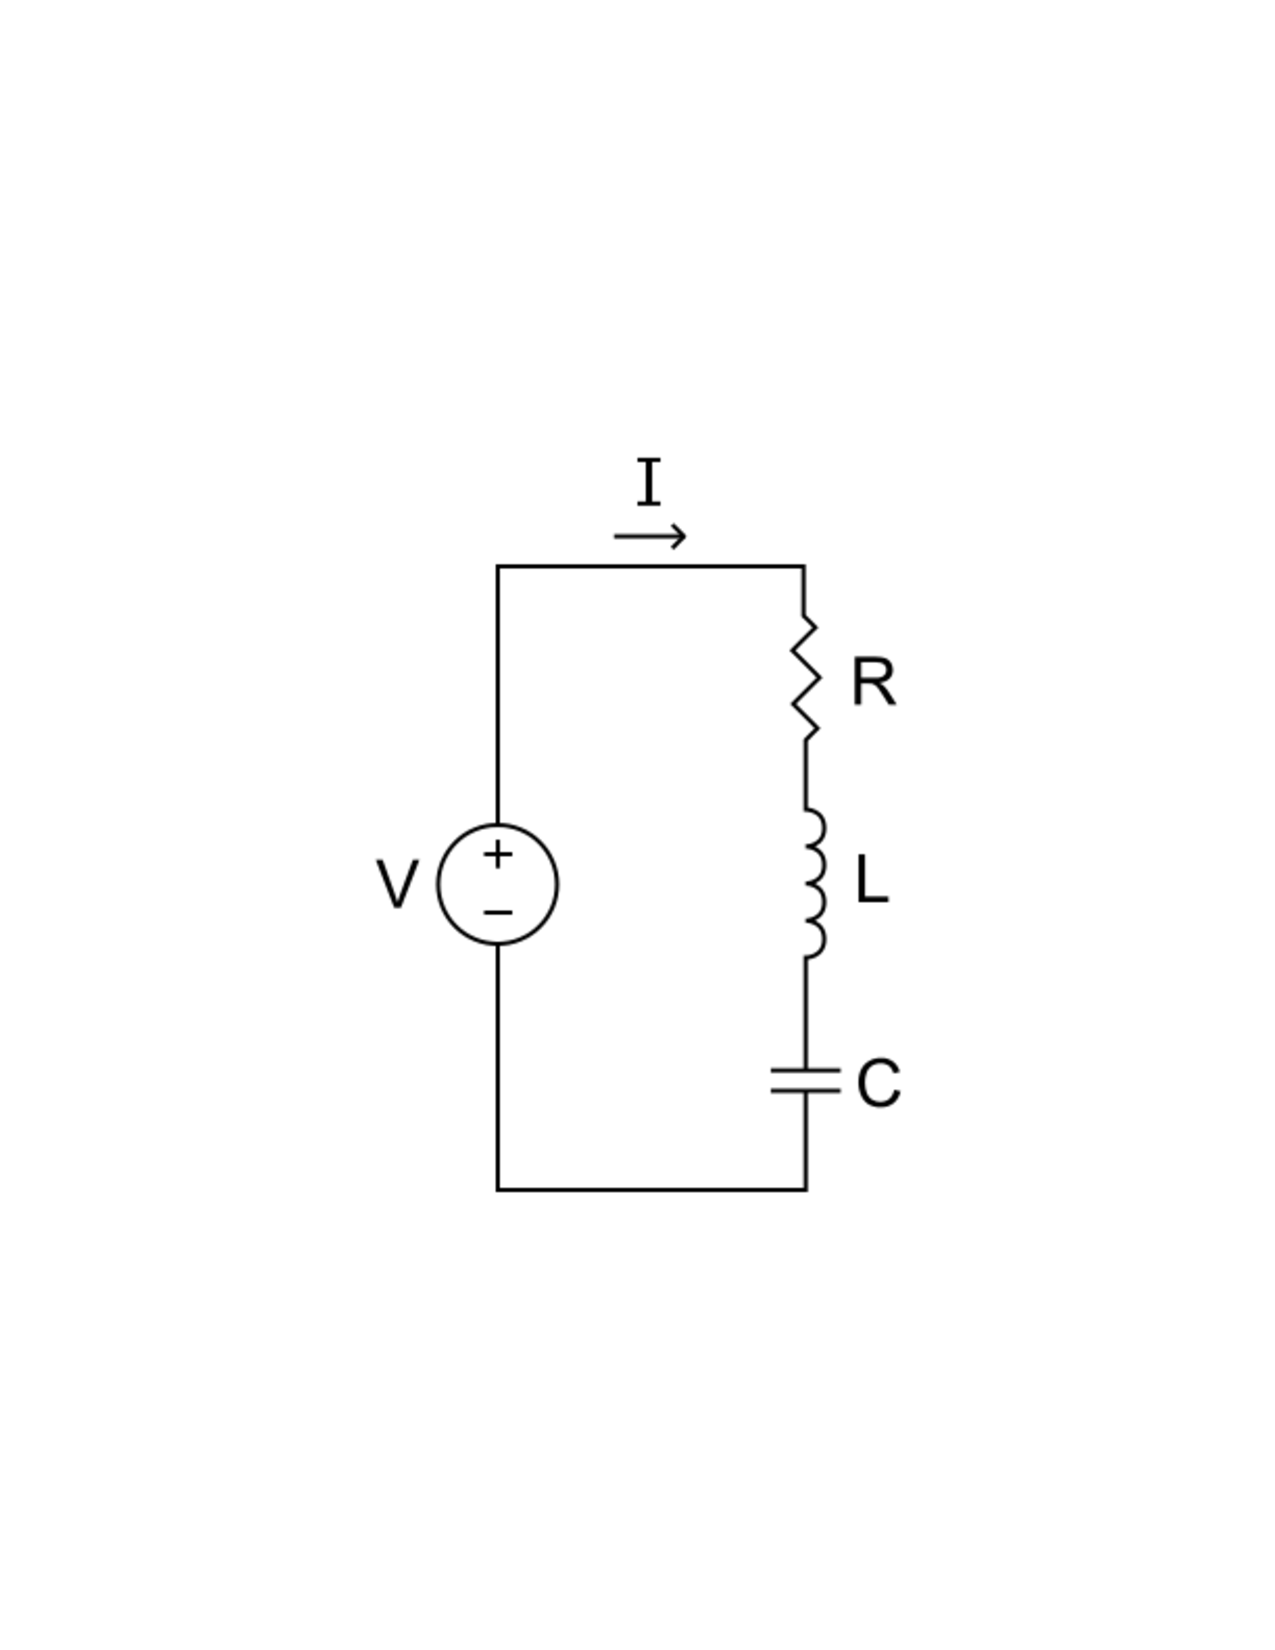
\includegraphics[width=0.15\textwidth,trim=6.25cm 7.75cm 6.25cm 7.75cm,clip]{RLC}
		\caption{An LCR series circuit~\cite{RLC}.}
		\label{LCR}
	\end{figure}
	
	For the complex susceptibility, we recall that differentiating in the time domain is equivalent to multiplying by $i \omg$ in the frequency domain~\cite{Fourier}:
	\eq{
		\cF_x [ f^{(n)}(x) ](\omg) = (i \omg)^n \cF [ f(x) ](\omg).
	}
	We Fourier transform both sides of Eq.~\refeq{ODE}:
	\eq{
		\Vomg = L (i \omg)^2 \qomg + R (i \omg) \qomg + \frac{\qomg}{C}
		= \paren{ i \omg R - \omg^2 L^2 + \frac{1}{C} } \qomg
		\qimplies
		\qomg = \frac{\Vomg}{i \omg R - \omg^2 L^2 + 1 / C}.
	}
	Applying Eq.~\refeq{susceptibility}, we find
	\eqn{chians}{
		\ans{ \chiomg = \frac{1}{i \omg R - \omg^2 L^2 + 1 / C}. }
	}
	\vfix
}



\prob{
	Show that the forced solution of this equation is
	\eq{
		\qt = \frac{\Vo \cos(\omg t - \phi)}{\sqrt{ (-\omg^2 L + 1 / C)^2 + (\omg R)^2 }},
	}
	where
	\eq{
		\tan(\phi) = \frac{\omg R}{\omg^2 L - 1 / C}.
	}
	\vfix
}

\sol{
	Equation~\refeq{ODE} is an ODE representing forced damped motion of a mass-spring system.  Its solution can be written as the sum of the homogeneous solution, which dies out with time, and a particular solution~\cite[pp.~38, 40, 50--51]{Olmstead}.  Rewriting Eq.~\refeq{ODE} as
	\eq{
		\frac{\Vo}{L} \cos(\omg t) = \qdd + 2 p \qd + \omgo^2 q
	}
	where $p = R / 2 L$ and $\omgo^2 = 1 / L C$, the ansatz for the particular solution is
	\eq{
		\qt = \Ac \cos(\omg t) + \As \sin(\omg t).
	}
	Feeding this into the ODE and collecting terms yields
	\al{
		-\Ac \omg^2 + 2 p \As \omg + \omgo^2 \Ac &= \frac{\Vo}{L}, &
		-\As \omg^2 - 2 p \Ac \omg + \omgo^2 \As &= 0.
	}
	This system has the solutions~\cite[p.~51]{Olmstead}
	\aln{ \label{AcAs}
		\As &= \frac{2 p \omg \Vo / L}{4 p^2 \omg^2 + (\omgo^2 - \omg^2)^2}, &
		\Ac &= \frac{(\omg^2 - \omgo^2) \Vo / L}{4 p^2 \omg^2 + (\omgo^2 - \omg^2)^2}.
	}
	If we define
	\eqn{A}{
		A = \sqrt{\Ac^2 + \As^2}
	}
	and write
	\eq{
		\qt = A \paren{ \frac{\Ac}{A} \cos(\omg t) + \frac{\As}{A} \sin(\omg t), }
	}
	there exists an angle $\phi$ such that $\cos(\phi) = \Ac / A$, $\sin(\phi) = \As / A$, and $\tan(\phi) = \As / \Ac$.  Thus
	\eq{
		\qt = A [ \cos(\phi) \cos(\omg t) + \sin(\phi) \sin(\omg).
	}
	Using the identity
	\eq{
		\cos(\alp) \cos(\bet) + \sin(\alp) \sin(\bet) = \cos(\alp - \bet),
	}
	it follows that~\cite[pp.~39, 51]{Olmstead}
	\eq{
		\qt = A \cos(\omg t - \phi).
	}
	The amplitude $A$ is given by~\cite[p.~51]{Olmstead}
	\al{
		A &= \frac{C \Vo}{\sqrt{(\nu^2 - 1)^2 + 4 c^2 \nu^2}}, &
		\qwhere
		c &= \frac{R}{2 \sqrt{L / C}}, \quad
		\nu = \frac{\omg}{\omgo}.
	}
	Substituting back to the original quantities, this is
	\eq{
		A = \frac{C \Vo}{\sqrt{(\omg^2 / \omgo^2 - 1)^2 + (R^2 C / L) (\omg^2 / \omgo^2) }} \\
		= \frac{C \Vo}{\sqrt{(L C \omg^2 - 1)^2 + C^2s R^2 \omg^2 }} \\
		= \frac{\Vo}{\sqrt{ (-\omg^2 L + 1 / C)^2 + (\omg R)^2 }}.
	}
	Additionally, from $\tan(\phi) = \As / \Ac$,
	\eq{
		\tan(\phi) = \frac{2 p \omg}{\omg^2 - \omg0^2}
		= \frac{R \omg / L}{\omg^2 - 1 / L C}
		= \ans{ \frac{\omg R}{\omg^2 L - 1 / C}. }
	}
	Hence we have shown
	\eq{
		\ans{ \qt = \frac{\Vo \cos(\omg t - \phi)}{\sqrt{ (-\omg^2 L + 1 / C)^2 + (\omg R)^2 }} }
	}
	as desired. \qed
}



\prob{
	Show that the mean rate of power dissipation is
	\eq{
		W = \frac{1}{2} \frac{ \omg \Vo^2 \sin(\phi)}{\sqrt{ (-\omg^2 L + 1 / C)^2 + (\omg R)^2 }}.
	}
}

\sol{
	The average power into a general AC circuit is~\cite[p.~1032]{YF}
	\eq{
		\Pav = \frac{1}{2} V I \sin(\phi),
	}
	where $I$ is the current amplitude, $V$ is the voltage amplitude, and $\phi$ is the phase angle determined in \ref{1a}~\cite[pp.~1028, 1032]{YF}.  Assuming the circuit is perfectly efficient, the average power into the circuit is equal to the average power it dissipates, so $W = \Pav$.  Clearly $V = \Vo$.  For I,
	\eqn{chi1}{
		\It = \dv{\qt}{t}
		= \dv{t}( \frac{\Vo \cos(\omg t - \phi)}{\sqrt{ (-\omg^2 L + 1 / C)^2 + (\omg R)^2 }} )
		= -\frac{\omg \Vo \sin(\omg t - \phi)}{\sqrt{ (-\omg^2 L + 1 / C)^2 + (\omg R)^2 }},
	}
	so
	\eqn{chi2}{
		I = \frac{\omg \Vo}{\sqrt{ (-\omg^2 L + 1 / C)^2 + (\omg R)^2 }}.
	}
	Thus
	\eqn{chi3}{
		W = \frac{1}{2} V I \sin(\phi) = \ans{ \frac{1}{2} \frac{ \omg \Vo^2 \sin(\phi)}{\sqrt{ (-\omg^2 L + 1 / C)^2 + (\omg R)^2 }} }
	}
	as we wanted to show. \qed
}



\prob{
	Sketch the real and imaginary parts of $\chi$ as a function of frequency, for the cases $Q \ll 1$, $Q \approx 1$, and $Q \gg 1$, where $Q = \sqrt{L / C} / R$ is the ``quality factor.''
	
	Where are the poles of $\chi$ in the complex $\omg$ plane?
}

\sol{
	From Eq.~\refeq{chians}, we can write $\chiomg$ in terms of $Q$ as
	\eq{
		\chiomg = \frac{1}{i \omg Q \sqrt{C / L} + Q^2 / R^2 L - \omg^2 Q^4 C^2 / R^4}.
	}
	In the case $Q \ll 1$, the Taylor series expansion to $\order{Q}$ is
	\eq{
		\chiomg \approx \frac{L^2}{C R^2 \omg^2} + i \paren{ \frac{Q L^3}{\omg^3 R^4 C \sqrt{C / L}} - \frac{1}{\omg Q \sqrt{C / L}} }
		= \frac{L^2}{\omg^2 C R^2} + i \paren{ \frac{L^4}{\omg^3 R^5 C^2} - \frac{L R}{\omg C} },
	}
	which we have evaluated using Mathematica.  In the case $Q \approx 1$,
	\eq{
		\chiomg \sim \frac{1}{i \omg R - \omg^2 L^2 + 1 / C}
	}
	so
	\al{
		\Re[ \chiomg ] &= \frac{1 / C - \omg^2 L^2}{(1 / C - \omg^2 L^2)^2 + \omg^2 R^2}, &
		\Im[ \chiomg ] &= -\frac{\omg R}{(1 / C - \omg^2 L^2)^2 + \omg^2 R^2}.
	}
	In the case $Q \gg 1$, the Taylor series expansion to $\order{Q^4}$ is
	\eq{
		\chiomg \approx -\frac{R^4}{\omg^2 Q^2 C^2}
		= -\frac{R^2}{\omg^2 L C},
	}
	which is real.
	
	Figure~\ref{1d} shows plots of the real~(blue line) and imaginary~(gold line) parts of $\chiomg$ in the cases $Q \ll 1$~(top left), $Q \approx 1$~(top right), and $Q \gg 1$~(bottom).
	
	\begin{figure}[t] \centering
		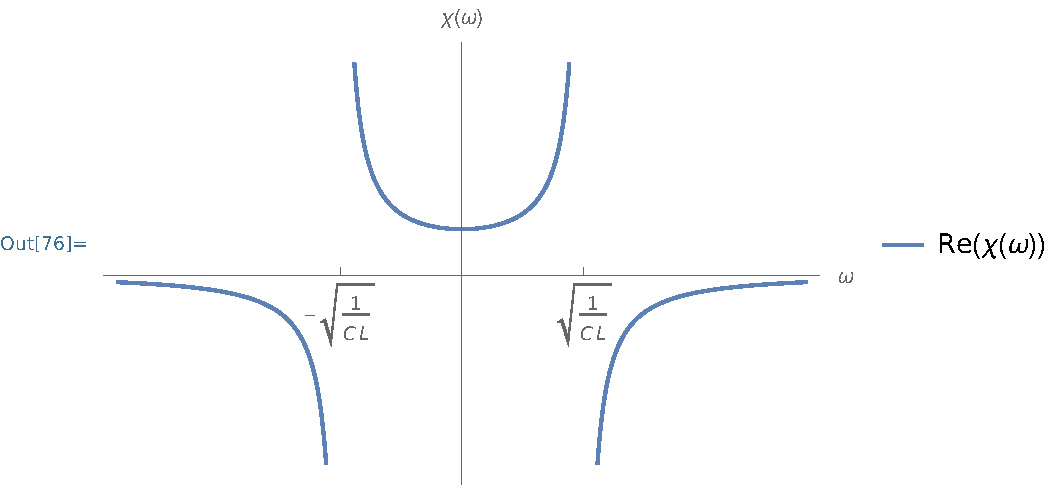
\includegraphics[width=0.49\textwidth,trim=1.5cm 0 0 0,clip]{1di} \hfill
		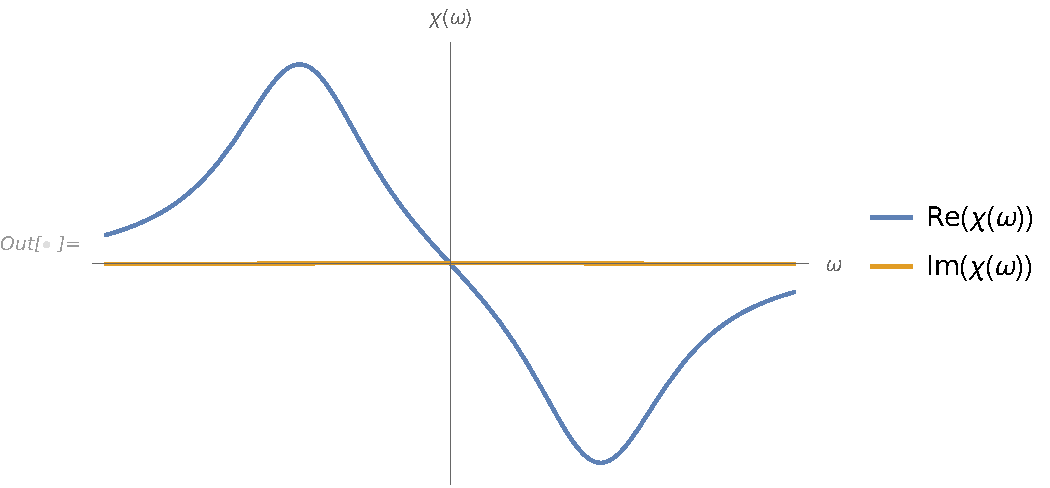
\includegraphics[width=0.49\textwidth,trim=1.5cm 0 0 0,clip]{1dii} \\[0.5cm]
		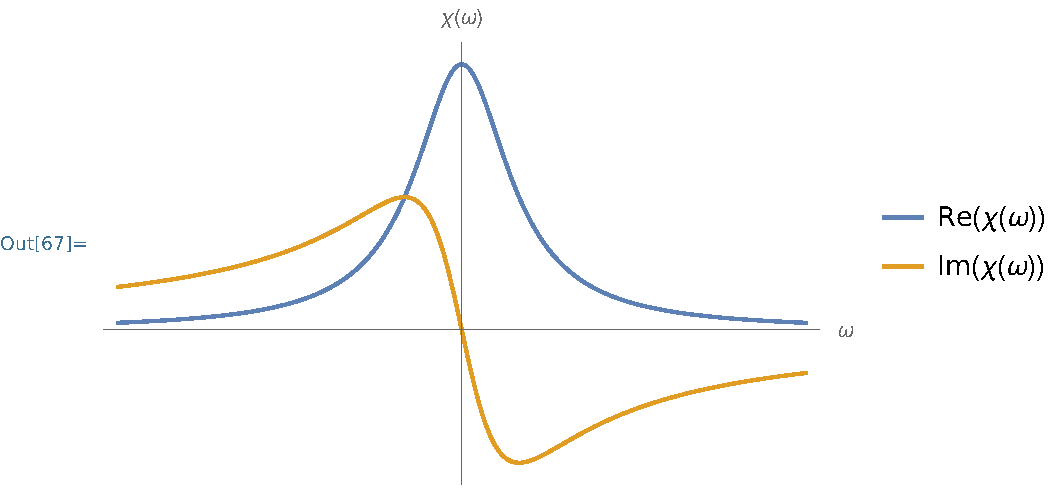
\includegraphics[width=0.49\textwidth,trim=1.5cm 0 0 0,clip]{1diii}
		\caption{Real~(blue line) and imaginary~(gold line) parts of $\chiomg$ in the cases $Q \ll 1$~(top left), $Q \approx 1$~(top right), and $Q \gg 1$~(bottom).  These cases are given by Eqs.~\refeq{chi1}, \refeq{chi2}, and \refeq{chi3}, respectively.}
		\label{1d}
	\end{figure}
	
	The function has poles at $\omgb$ such that $1 / \chiomgb = 0$~\cite{Poles}:
	\eq{
		0 = i \omgb R - \omgb^2 L^2 + \frac{1}{C}
		\qimplies
		\ans{ \omgb = \frac{i R \pm \sqrt{4 L^2 / C - R^2}}{2 L^2}. }
	}
	\vfix
}